\documentclass[crop,tikz]{standalone}
\usetikzlibrary{calc}
\usepackage{siunitx}
\begin{document}
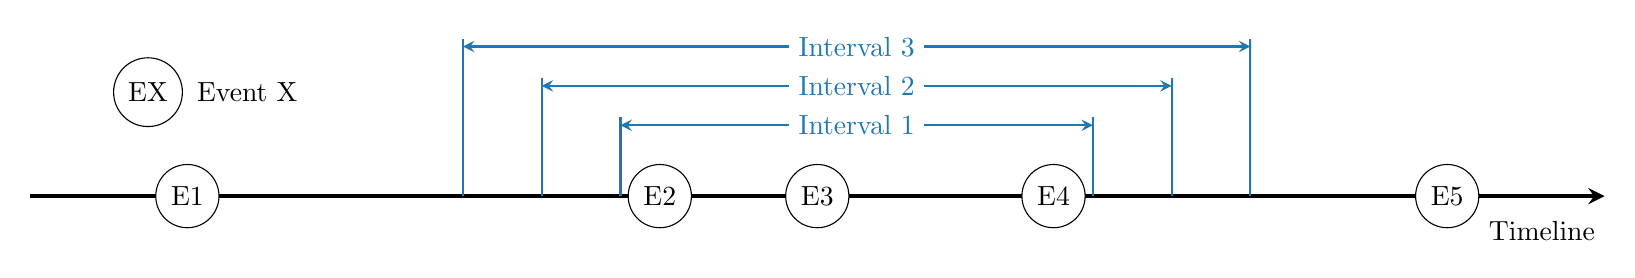
\begin{tikzpicture}
    \definecolor{C0}{HTML}{1f77b4}

    \path[draw, ultra thick, -stealth] (0,0) -- (20,0);

    \node[draw, shape=circle, fill=white] (e1) at (2,0) {E1};
    \node[draw, shape=circle, fill=white] (e2) at (8,0) {E2};
    \node[draw, shape=circle, fill=white] (e3) at (10,0) {E3};
    \node[draw, shape=circle, fill=white] (e4) at (13,0) {E4};
    \node[draw, shape=circle, fill=white] (e5) at (18,0) {E5};

    \node at (20,-0.2) [anchor=north east] {Timeline};

    \path[draw=C0, thick] ($ (e2) + (-0.5,0) $) -- ($ (e2) + (-0.5,1) $);
    \path[draw=C0, thick] ($ (e4) + (0.5,0) $) -- ($ (e4) + (0.5,1) $);
    \path[draw=C0, thick, stealth-stealth] ($ (e2) + (-0.5,0.9) $) -- node [fill=white] {\textcolor{C0}{Interval 1}} ($ (e4) + (0.5,0.9) $);

    \path[draw=C0, thick] ($ (e2) + (-1.5,0) $) -- ($ (e2) + (-1.5,1.5) $);
    \path[draw=C0, thick] ($ (e4) + (1.5,0) $) -- ($ (e4) + (1.5,1.5) $);
    \path[draw=C0, thick, stealth-stealth] ($ (e2) + (-1.5,1.4) $) -- node [fill=white] {\textcolor{C0}{Interval 2}} ($ (e4) + (1.5,1.4) $);

    \path[draw=C0, thick] ($ (e2) + (-2.5,0) $) -- ($ (e2) + (-2.5,2) $);
    \path[draw=C0, thick] ($ (e4) + (2.5,0) $) -- ($ (e4) + (2.5,2) $);
    \path[draw=C0, thick, stealth-stealth] ($ (e2) + (-2.5,1.9) $) -- node [fill=white] {\textcolor{C0}{Interval 3}} ($ (e4) + (2.5,1.9) $);

    \begin{scope}[xshift=1.5cm, yshift=1.2cm]
        \node[draw, shape=circle, anchor=base] (ex) at (0,0) {EX};
        \node at (0.5,0) [anchor=base west] {Event X};
    \end{scope}


\end{tikzpicture}
\end{document}
